\documentclass{article}
\usepackage{tikz}
\usetikzlibrary{calc,fadings,decorations.pathreplacing}
\begin{document}
	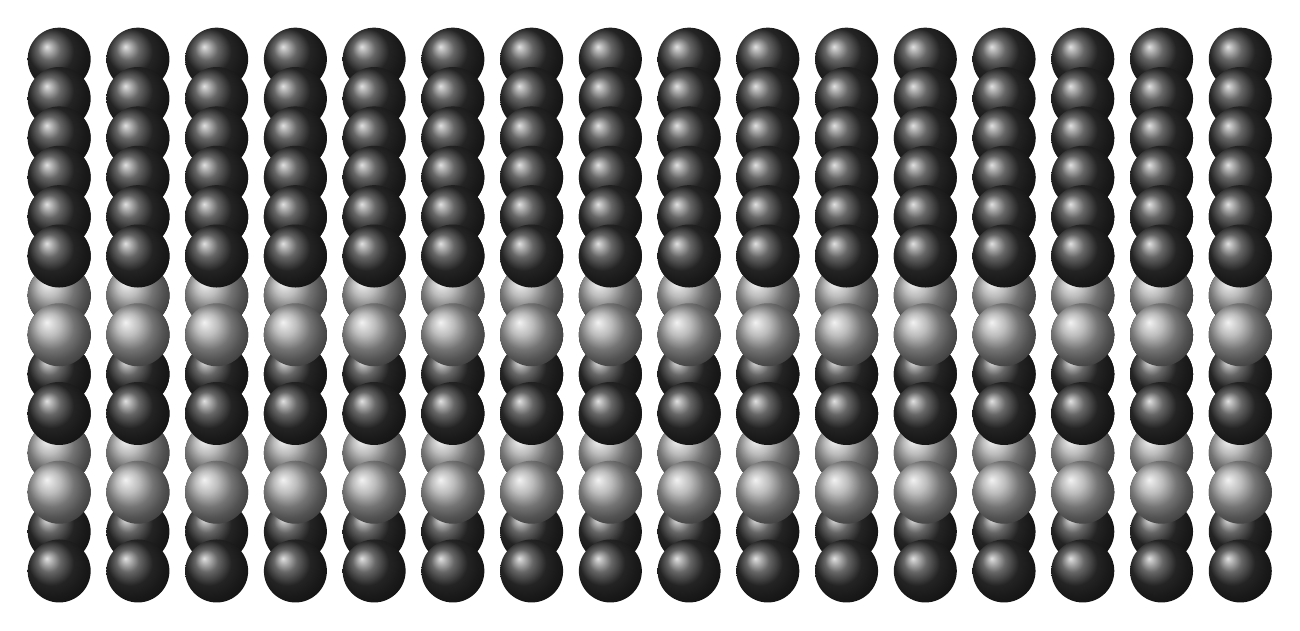
\begin{tikzpicture}
		\def\nuPi{3.1459265}
		\foreach \i in {15,14,...,0}{% This one doesn't matter
			\foreach \j in {5,4,...,0}{% This will crate a membrane
									% with the front lipids visible
			% top layer
			\pgfmathsetmacro{\dx}{0.5}% A random variance in the x coordinate
			\pgfmathsetmacro{\dy}{0.5}% A random variance in the y coordinate,    
			\shade[ball color=black!80] (\i+\dx,{0.5*\j+\dy+ 4} ) circle(0.4);
			\shade[ball color=gray!70] (\i+\dx,{0.5*\j+\dy+ 3}) circle(0.4);
			% bottom layer
			\pgfmathsetmacro{\dx}{0.5}
			\pgfmathsetmacro{\dy}{0.5}
			\shade[ball color=black!80] (\i+\dx,{0.5*\j+\dy+2}) circle(0.4);
			\shade[ball color=gray!70] (\i+\dx,{0.5*\j+\dy+1}) circle(0.4);
			\shade[ball color=black!80] (\i+\dx,{0.5*\j+\dy+0}) circle(0.4);
			}
		}
	\end{tikzpicture}
\end{document}

% \documentclass{article}

% \usepackage{tikz}

% \usetikzlibrary{patterns}
% \usetikzlibrary{perspective}


% \newcommand\simplecuboid[3]{%
% 	\fill[pattern = checkerboard, pattern color = gray!80] (tpp cs:x=0,y=0,z=#3)
% 	-- (tpp cs:x=0,y=#2,z=#3)
% 	-- (tpp cs:x=#1,y=#2,z=#3)
% 	-- (tpp cs:x=#1,y=0,z=#3) -- cycle;
% 	\fill[pattern = checkerboard, pattern color = gray!60] (tpp cs:x=0,y=0,z=0)
% 	-- (tpp cs:x=0,y=0,z=#3)
% 	-- (tpp cs:x=0,y=#2,z=#3)
% 	-- (tpp cs:x=0,y=#2,z=0) -- cycle;
% 	\fill[pattern = checkerboard, pattern color = gray!40] (tpp cs:x=0,y=0,z=0)
% 	-- (tpp cs:x=0,y=0,z=#3)
% 	-- (tpp cs:x=#1,y=0,z=#3)
% 	-- (tpp cs:x=#1,y=0,z=0) -- cycle;}
% \newcommand{\simpleaxes}[3]{%
% 	\draw[->] (0,0,0) -- (#1,0,0) node[pos=1.1]{x};
% 	\draw[->] (0,0,0) -- (0,#2,0) node[pos=1.1]{y};
% 	\draw[->] (0,0,0) -- (0,0,#3) node[pos=1.1]{z};}

% \begin{document}
% 	\begin{tikzpicture}[3d view]
% 		\simplecuboid{10}{2}{2}
% 		\simpleaxes{11}{3}{3}
		
% 	\end{tikzpicture}
% \end{document}
